%%%%%%%%%%%%%%%%%%%%%%%%%%%%%%%%%%%%%%%%%
% University Assignment Title Page 
% LaTeX Template
% Version 1.0 (27/12/12)
%
% This template has been downloaded from:
% http://www.LaTeXTemplates.com
%
% Original author:
% WikiBooks (http://en.wikibooks.org/wiki/LaTeX/Title_Creation)
%
% License:
% CC BY-NC-SA 3.0 (http://creativecommons.org/licenses/by-nc-sa/3.0/)
% 
% Instructions for using this template:
% This title page is capable of being compiled as is. This is not useful for 
% including it in another document. To do this, you have two options: 
%
% 1) Copy/paste everything between \begin{document} and \end{document} 
% starting at \begin{titlepage} and paste this into another LaTeX file where you 
% want your title page.
% OR
% 2) Remove everything outside the \begin{titlepage} and \end{titlepage} and 
% move this file to the same directory as the LaTeX file you wish to add it to. 
% Then add \input{./title_page_1.tex} to your LaTeX file where you want your
% title page.
%
%%%%%%%%%%%%%%%%%%%%%%%%%%%%%%%%%%%%%%%%%

%----------------------------------------------------------------------------------------
%	PACKAGES AND OTHER DOCUMENT CONFIGURATIONS
%----------------------------------------------------------------------------------------

\documentclass[12pt]{article}

\usepackage{graphicx}
\usepackage{subcaption}
\usepackage[usenames, dvipsnames]{color}

\begin{document}

\begin{titlepage}

\newcommand{\HRule}{\rule{\linewidth}{0.5mm}} % Defines a new command for the horizontal lines, change thickness here

\center % Center everything on the page
 
%----------------------------------------------------------------------------------------
%	HEADING SECTIONS
%----------------------------------------------------------------------------------------

\textsc{\LARGE Barcelona Graduate School}\\[0.2cm] % Name of your university/college
\textsc{\LARGE of Economics}\\[1.5cm] % Name of your university/college
\textsc{\Large Masters Project}\\[0.5cm] % Major heading such as course name
\textsc{\large }\\[0.5cm] % Minor heading such as course title

%----------------------------------------------------------------------------------------
%	TITLE SECTION
%----------------------------------------------------------------------------------------

\HRule \\[0.4cm]
{ \huge \bfseries Combinatorial Bandit}\\[0.4cm] % Title of your document
{ \huge \bfseries Algorithms in Practice}\\[0.4cm]
\HRule \\[1.5cm]
 
%----------------------------------------------------------------------------------------
%	AUTHOR SECTION
%----------------------------------------------------------------------------------------

%\begin{minipage}{0.4\textwidth}
%\begin{flushleft} \large
%\emph{Authors:}\\
%Angus \textsc{McKay} % Your name
%Akhil \textsc{Lohia} % Your name
%\end{flushleft}
%\end{minipage}
%~
%\begin{minipage}{0.4\textwidth}
%\begin{flushright} \large
%\emph{Supervisor:} \\
%Dr. James \textsc{Smith} % Supervisor's Name
%\end{flushright}
%\end{minipage}\\[4cm]

% If you don't want a supervisor, uncomment the two lines below and remove the section above
\Large \emph{Authors:}\\
Angus \textsc{McKay}\\ % Your name
Akhil \textsc{Lohia}\\[3cm] % Akhil's name

%----------------------------------------------------------------------------------------
%	DATE SECTION
%----------------------------------------------------------------------------------------

{\large \today}\\[3cm] % Date, change the \today to a set date if you want to be precise

%----------------------------------------------------------------------------------------
%	LOGO SECTION
%----------------------------------------------------------------------------------------

%\includegraphics{Logo}\\[1cm] % Include a department/university logo - this will require the graphicx package
 
%----------------------------------------------------------------------------------------

\vfill % Fill the rest of the page with whitespace

\end{titlepage}

%----------------------------------------------------------------------------------------
%	ABSTRACT PAGE
%----------------------------------------------------------------------------------------

\section{Abstract}
%\addchaptertocentry{\abstractname} % Add the abstract to the table of contents


There has recently been a lot of interest in online learning algorithms where limited feedback is received at each stage of the process, known as bandit problems. Such algorithms generally choose a subset of available options to 'play' at each round. For the options chosen, some stochastic reward (or cost) is returned. In a semi-bandit situation, the reward is observed for each option which is played. In a full-bandit scenario, only the total reward is observed. A lot of practical problems also contain a combinatorial element to them, whereby a combinatorial problem needs to be solved using the feedback observed.\\

Recent literature has proposed many different algorithms and approaches for these bandit problems. The literature is also full of mathematical proofs for bounds on regret risk (i.e. the difference between a chosen solution and the optimal solution). However, there is relatively little information on how these algorithms perform in practice. This paper intends to explore the performance of some of the proposed approaches in a more practical setting. 

\pagebreak

\vfill % Fill the rest of the page with whitespace

%----------------------------------------------------------------------------------------
%	ACKNOWLEDGEMENTS
%----------------------------------------------------------------------------------------

\section{Acknowledgements}
%\addchaptertocentry{\acknowledgementname} % Add the acknowledgements to the table of contents
The acknowledgments and the people to thank go here

\pagebreak

%----------------------------------------------------------------------------------------
%	LIST OF CONTENTS/FIGURES/TABLES PAGES
%----------------------------------------------------------------------------------------

\tableofcontents % Prints the main table of contents

\pagebreak

%----------------------------------------------------------------------------------------
%	INTRO
%----------------------------------------------------------------------------------------

\section{Introduction}

\subsection{Online learning}

In the online learning environment, a 'player' has a selection of options that they can choose from. Once an option is selected the environment provides some cost or reward. The player then has a decision whether to continue with the selected option or to try something different. It is usually a good idea to explore the different options available before exploiting the best ones. There has recently been a lot of interest in developing strategies for addressing this exploration vs exploitation.\\

In the simplest scenario, the feedback received is \textbf{deterministic}. In this case if one can explore all of the options available then the full environment is known and there is know more learning needed. A more difficult problem is when the feedback is instead \textbf{stochastic} in nature. At each iteration some feedback on the chosen option provides some further insight into the environment, but the actual outcome will never be known for certain. One can try to figure out the best option at each iteration in order to reduce/maximise the expected cost/reward. Various algorithms have been proposed for the stochastic situation which allow one to place an upper bound on the "regret" (or sometimes Bayesian regret) of the system, where regret is defined as the difference in cost/reward between the chosen options and the optimal option.\\

An even more challenging scenario is when the costs/rewards are \textbf{adversarial}. This situation has stochastically drawn feedback from the envirnoment, but the distributions which the feedback is drawn from is not necessarily the same at each iteration. Amazingly, there are algorithms which, given certain constraints on the environment, can still provide upper bounds on the regret risk. These algorithms keep up their exploration aspect in order to adapt to new optimal solutions arising as the situation changes.

\subsection{Combinatorial bandit}

Combinatorial element and optimization oracle

Exploration vs exploitation

Examples


\pagebreak

%----------------------------------------------------------------------------------------
%	ALGORITHMS
%----------------------------------------------------------------------------------------

\section{Algorithms}

\subsection{CombUCB1}

One of the most well-known algorithms for multi-armed bandit problems is UCB1. This has been adapted to the combinatorial setting by Kveton et al [1], who developed CombUCB1. After each iteration the algorithm calculates a confidence bound around the empirical mean reward/cost of each element. These confidence bounds are then used in the combinatorial optimization problem, the solution of which is the chosen play for the next round. The more observations that are available of an element, the tighter the confidence bound around the expeceted value. Loosely speaking, relatively unobserved items will have larger confidence bounds so they will be explored until there is more confidence in their expected value.\\

The confidence intervals at time $t$ are calculated as:

$$\hat{w}_{t-1}(e)\pm c_{t-1,e}$$ where $\hat{w}_{t-1}(e)$ is the average of the observations of option $e$ up to time $t-1$. $c_{t-1,e}$ is calculated as:

$$c_{t-1,e}=\sqrt{\frac{1.5\textrm{log}(t-1)}{n_{t-1}(e)}}$$ where $n_{t-1}(e)$ is the number of times that option $e$ has been observed up to time $t-1$.\\

The algorithm is set out formally below.

\noindent \hrulefill

\noindent \textbf{CombUCB1} algorithm for combinatorial semi-bandit problems

\noindent \hrulefill

\noindent \textit{Initialization}:

$\mathbf{\hat{w}}_0 \leftarrow$ make one observation of each edge

$n_0(e) \leftarrow 1$ $\forall$ $e \in E$\\

\noindent \textit{For all t in 1,...,T}:

Compute confidence intervals for each edge:

\indent \indent $U_t(e) \leftarrow \hat{w}_t(e)\pm c_{t-1,e}$ $\forall$ $e \in E$\\

Solve the optimization problem:

\indent \indent $A_t \leftarrow \textrm{arg max}_{A\in \Theta}f(A,U_t)$\\

Observe the weights of chosen items:

\indent \indent $w_t(e) \sim P_e$ $\forall$ $e \in A_t$

\indent \indent $w_t(e)=0$ otherwise\\

Update counts and expected values for each edge:

\indent \indent $n_t(e) \leftarrow n_{t-1}(e) + 1$ $\forall$ $e \in A_t$

\indent \indent $\hat{w}_t(e) \leftarrow \frac{n_{t-1}(e)\hat{w}_{t-1}(e)+w_t(e)}{n_t(e)}$ $\forall$ $e \in E$

\noindent \hrulefill\\

This assumes that one is able to initialize by choosing to observe each edge at least once before starting the algorithm. In practice if this is not feasible then the algorithm will produce a similar output if the initial weight for each edge is assumed to be the maximum (if a maximization problem) or minimum (if a minimization problem) values of the system (but these initial values are then disregarded in the algorithm once an observation has been made).\\

Note that the algorithm is computationally efficient, provided that the combinatorial optimization can be solved efficiently. All other operations are polynomial in L and K.\\

TO DO - MAKE SURE EVERYTHING IS DEFINED PROPERLY EARLIER ON


FPL-TRiX

Others

Mathematical results (bounds etc)	


\pagebreak

%----------------------------------------------------------------------------------------
%	BASIC TESTING
%----------------------------------------------------------------------------------------

\section{Basic Testing}

\subsection{Basic stochastic setting}

For some initial insight into how the algorithms work in practice we can set up a basic simulation with a trivial combinatorial element. In this scenario we will have a vector of length L, and at each round K elements of this vector will be chosen. The weights of each chosen element will then be drawn from a Bernoulli distribution with a different mean for each element. A real-life application of such a system could be arranging adverts on a website where only K out of L adverts can be shown at any one time, and the goal is to maximise the number of times a user clicks on a link in an advert.\\

We start by setting L = 20, K = 5 and set the means as incrementally increasing values from 1/20 for the first element to 1 for the last element (so they are 1/20, 2/20, ..., 18/20, 19/20, 1). The game is to maximise the weights observed at each round. Clearly the optimal elements to play at each round are the last 5 elements as they have the highest probability of being drawn as 1. Let us observe how the algorithms explore the different options at different stages.\\


\noindent \textbf{UCB1}\\



\begin{figure}[h!]
\centering
\begin{subfigure}{.33\textwidth}
  \centering
  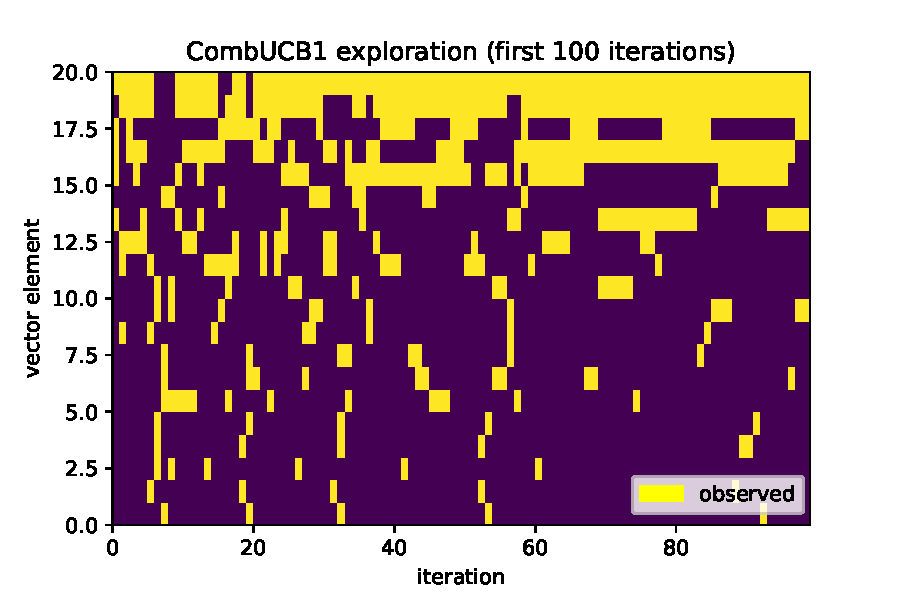
\includegraphics[width=50mm]{../plots/basicCombUCB1_100iters.pdf}
\end{subfigure}%
\begin{subfigure}{.33\textwidth}
  \centering
  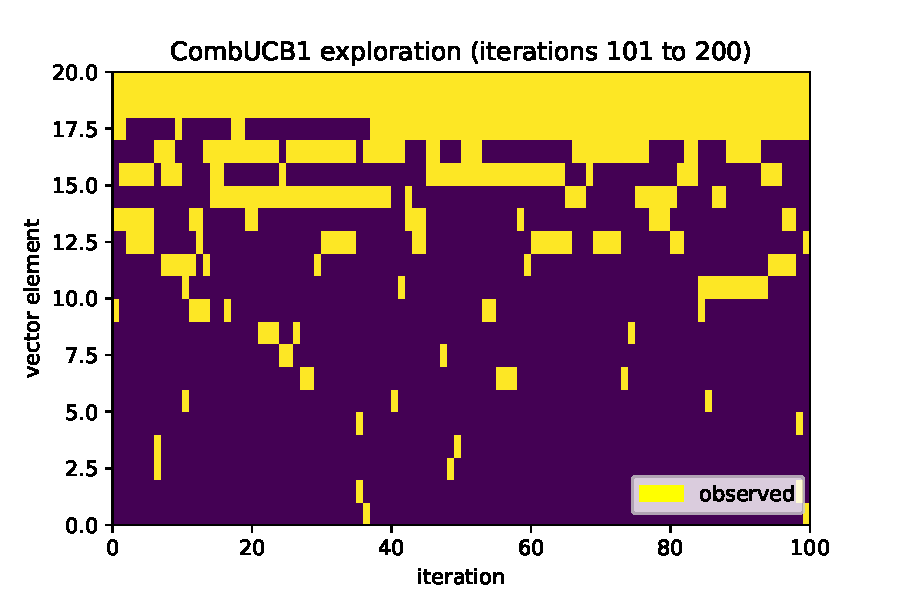
\includegraphics[width=50mm]{../plots/basicCombUCB1_100_200iters.pdf}
\end{subfigure}
\begin{subfigure}{.33\textwidth}
  \centering
  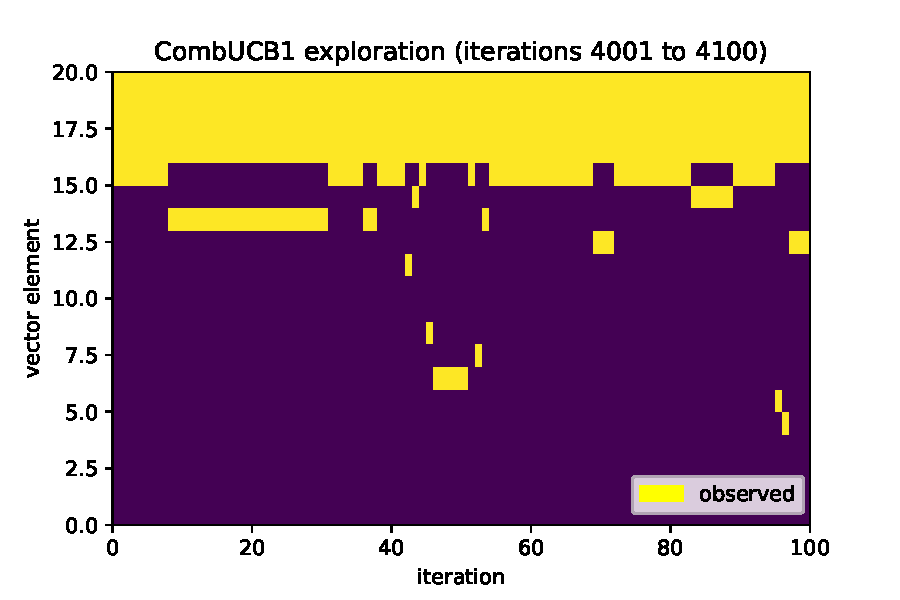
\includegraphics[width=50mm]{../plots/basicCombUCB1_4000_4100iters.pdf}
\end{subfigure}
\caption{CombUCB1 exploration at different stages}
\label{fig:ullm-particle}
\end{figure}

Figure XXX shows how at the outset the algorithm is not confident what the expected value of any of the weights are and so it explores a lot. Figure XXX shows iterations 101 to 200, when the algorithm is starting to learn which elements have the highest expected value. Finally Figure XXX shows the algorithm after 4000 iterations at which time is has become quite confident which are the optimal paths, and does relatively little exploration.\\

The regret risk can be calculated as the sum of observed weights minus the sum of the weights of the top 5 elements of the vector. For 10,000 iterations this gives the following:\\

Optimal path reward = 42,399

Actual path reward = 41,905

Regret = 494\\

The algorithm performs very well at finding a near optimal solution.\\

\noindent \textbf{Adapted-FPL-TRiX}\\

Figure XXX shows the corresponding charts for FPL-TRiX but adapted to find a maximum solution as opposed to a minimum solution. NEED MORE EXPLANATION HERE ONC ALGORITHM IS WRITTEN ABOVE In fact, by finding a maximum, this misses part of the essence of FPL-TRiX, which is that it adapts well in adversarial cases by keeping more of an open mind about trying the different options even once it has started to recognise the optimal solution. However, even though this is not exactly FPL-TRiX, it is interesting to include here as, with a bit of parameter tuning, it performs incredibly well in this situation. The reward and regret are:\\

Optimal path reward = 42,399

Actual path reward = 42,246

Regret = 153\\

Thus the algorithm outperforms CombUCB1. If we think of this slightly modified FPL-TRiX as part of the family of FPL-TRiX then it shows that this can be a nice adaptable framework to work in.\\

\begin{figure}[h!]
\centering
\begin{subfigure}{.33\textwidth}
  \centering
  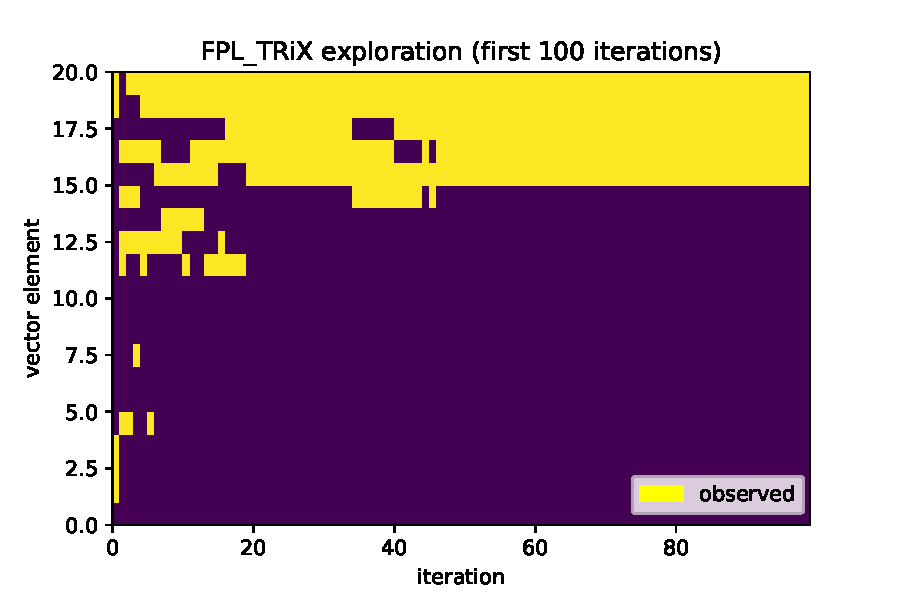
\includegraphics[width=50mm]{../plots/basicFPL_100iters.pdf}
\end{subfigure}%
\begin{subfigure}{.33\textwidth}
  \centering
  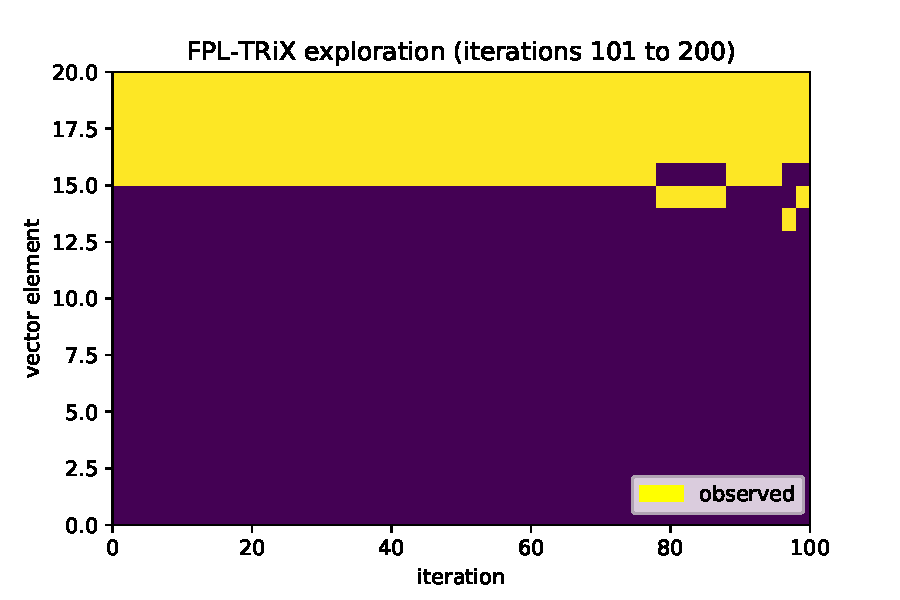
\includegraphics[width=50mm]{../plots/basicFPL_100_200iters.pdf}
\end{subfigure}
\begin{subfigure}{.33\textwidth}
  \centering
  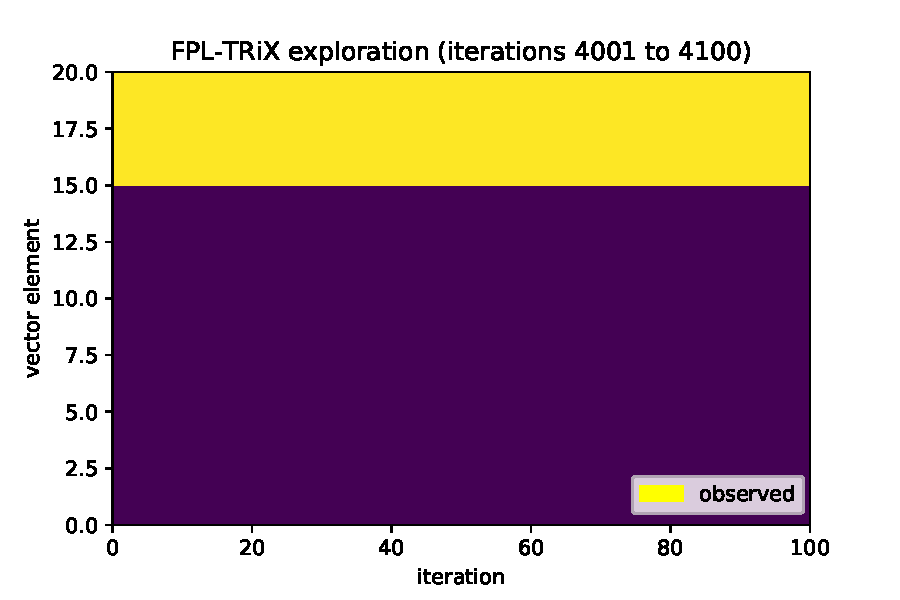
\includegraphics[width=50mm]{../plots/basicFPL_4000_4100iters.pdf}
\end{subfigure}
\caption{Adapted-FPL-TRiX exploration at different stages}
\label{fig:ullm-particle}
\end{figure}




DO WE WANT TO ALSO SHOW WHAT THE MATHEMATICAL BOUNDS ARE HERE???

Graphs showing how regret changes as inputs change (K, L, T etc)

Include adversarial case here?


\pagebreak

%----------------------------------------------------------------------------------------
%	NETWORK MINIMUM COST PATH PROBLEMS
%----------------------------------------------------------------------------------------

\section{Network minimum cost path problems}

A more sophisticated combinatorial problem to solve is a minimum cost path problem in a network. In this framework there are V vertices with edges in both directions between each pair of vertices, giving V $\times$ (V-1) edges in total (in practice if an edge does not exist between two vertices then the cost of the edge can be set to infinity). A path is chosen to travel from some starting vertex to an end vertex. The cost of each edge in the path is then stochastically drawn and the sum of these provides the total cost of the chosen path. The goal is to find the path with minimum expected cost. Clear application of this type of system in real-life could be any type of mass scale distibution such as electricity or communication networks.\\

Given the more difficult combinatorial problem, this pushes the Algorithms harder. They will need to work out which higher cost edges are beneficial to use in order to take advantage of low cost paths than lead into or out of them. Thus the relative level of regret should be much higher than the previous more basic problem.\\

\subsection{Stochastic networks}

Firstly we look at how CombUCB1 and FPL-TRiX perform in the stochastic setting, where the weights of the edges are drawn from truncated normal distributions limited to being between 0 and 1. Each edge has a different central point (i.e. different mean), and the variance was kept low at 0.1 so that there is a meaningful difference between the different paths.\\

With 10 vertices and observing 10,000 iterations the following costs were observed. This was after tuning the FPL-TRiX parameters, in particular reducing the gamma parameter to 0.01.\\

Optimal path cost = 2,269

UCB path cost = 3,742

FPL-TRiX path cost = 2,735\\

Perhaps surprisingly, FPL-TRiX is able to significantly outperform CombUCB1 in this situation. Figure XXX shows the edges of the optimal path at each iteration, and the edges of the paths chosen by CombUCB1 and FPL-TRiX. FPL-TRiX explores more at first allowing it to find the optimal path more quickly, whereas CombUCB1 is led towards shorter paths at first. If all edges start with similar wide confidence intervals then the paths with the least number of edges will appear to have the lowest costs. It is only after some time (around 200 iterations in this case) that CombUCB1 finds accurate enough estimates of the edges to work out that a longer path is in fact the optimal.\\

\begin{figure}[h!]
\centering
\begin{subfigure}{.33\textwidth}
  \centering
  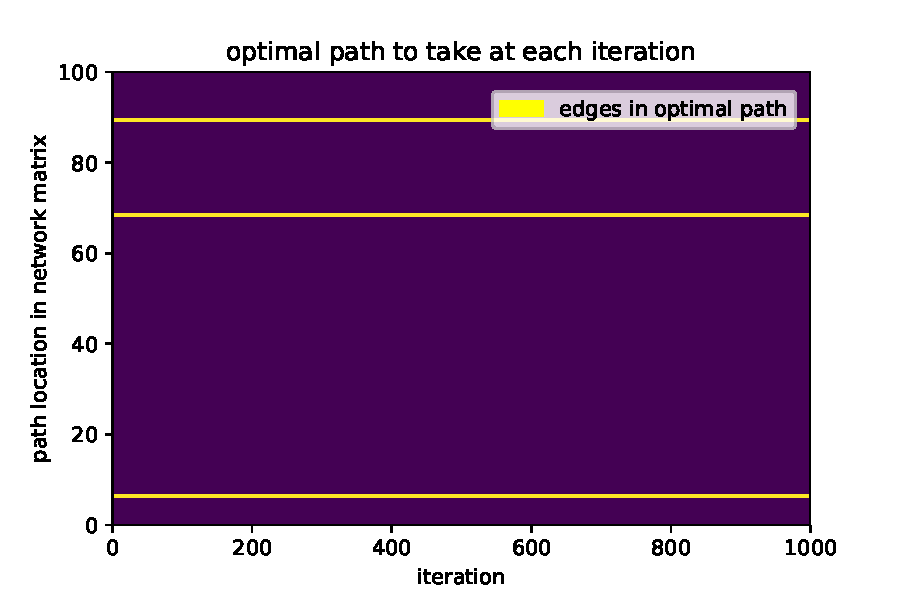
\includegraphics[width=50mm]{../plots/stoch_network_opt_paths.pdf}
\end{subfigure}%
\begin{subfigure}{.33\textwidth}
  \centering
  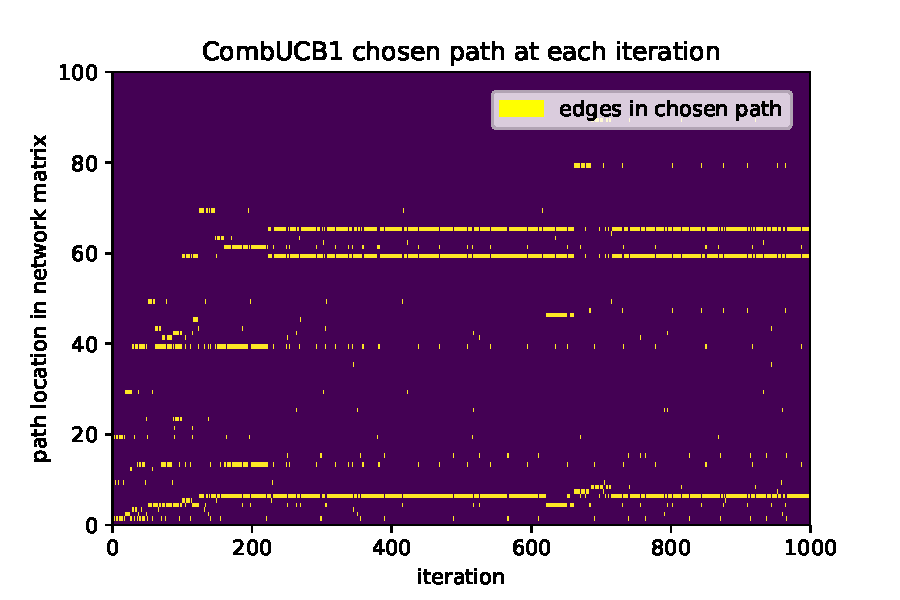
\includegraphics[width=50mm]{../plots/stoch_network_UCB1.pdf}
\end{subfigure}
\begin{subfigure}{.33\textwidth}
  \centering
  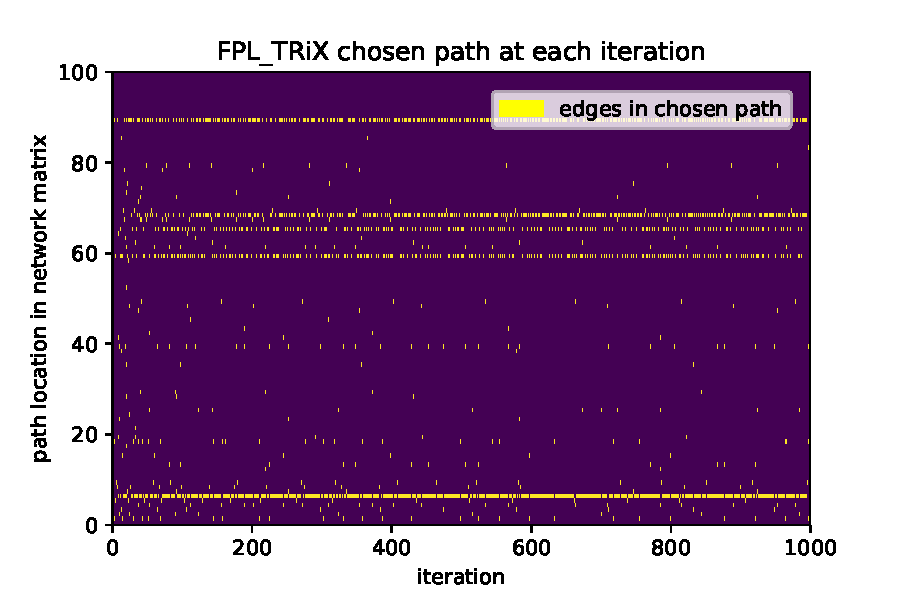
\includegraphics[width=50mm]{../plots/stoch_network_FPL.pdf}
\end{subfigure}
\caption{Optimal paths, CombUCB1 chosen paths and FPL-TRiX chosen paths}
\label{fig:ullm-particle}
\end{figure}


\subsection{Adversarial networks}

In this section we will progress to analysing the performance of the algorithms in an adversarial setting. To do this we continue the minimum cost path setting of the previous section, but allow the weights of the edges to be drawn from different distributions over different periods. The following three different settings were investigated\\

\subsubsection{Adversarial network 1 - long to short optimal path}

The first adversarial network we analyse starts with the optimal path being to visit each vertex sequentially from the first vertex to the last. Thus with 10 vertices the initial optimal path is nine edges long. After 5,000 iterations the optimal path changes to a shorter path of only two edges. The mean weights of the edges are shown in the network matrices in figure XXX. Element (i,j) of each matrix represents the mean of the truncated normal distribution that the weight of the edge from vertex i to j is drawn from at each iteration. In figure XXX the shortest path is from vertex 0 to 3 and then from 3 to 9\\

\begin{figure}[h!]
\centering
\begin{subfigure}{1.0\textwidth}
  \centering
  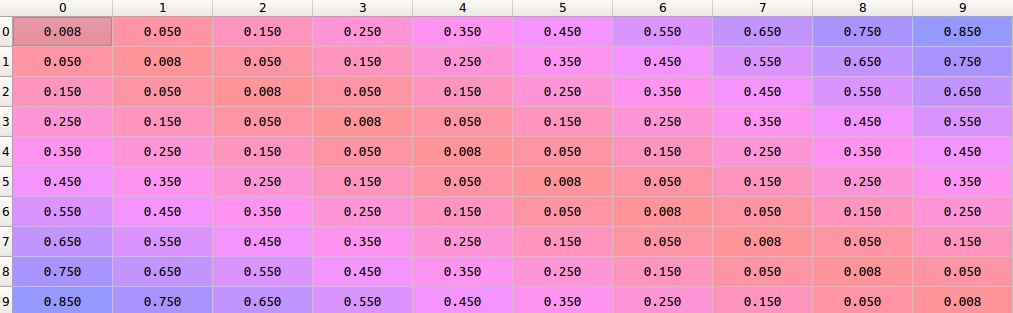
\includegraphics[width=14cm]{../plots/path_means1.png}
  \caption{Adversarial netrork 1 - initial mean edge weights}
  \label{}
  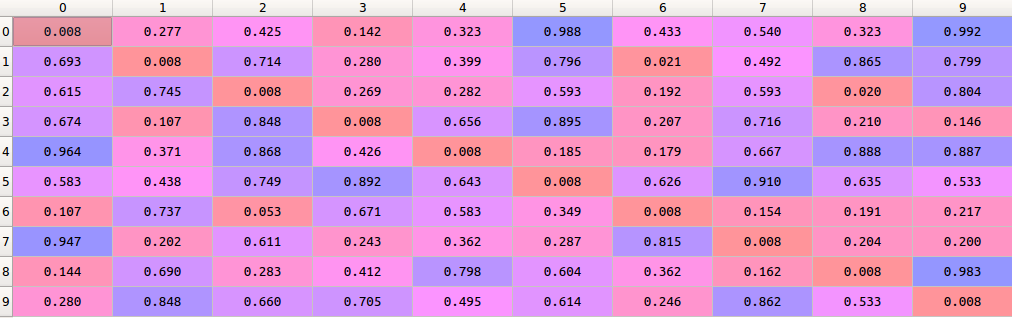
\includegraphics[width=14cm]{../plots/path_means2.png}
  \caption{Adversarial network 1 - second phase mean edge weights}
  \label{}
\end{subfigure}
\caption{Adversarial network 1 mean path weights at each phases}
\label{fig:ullm-particle}
\end{figure}


\subsubsection{Adversarial network 2 - short to long optimal path}

The second adversarial network is similar to the first but in reverse, whereby at first the optimal path is the shortest path, i.e. one edge straight from the first to the last vertex. After 1,000 iterations the optimal paths changes to one with many edges. The network alternates between these two situations every 1,000 iterations. The mean weights of the edges are shown in figure XXX.\\

\begin{figure}[h!]
\centering
\begin{subfigure}{1.0\textwidth}
  \centering
  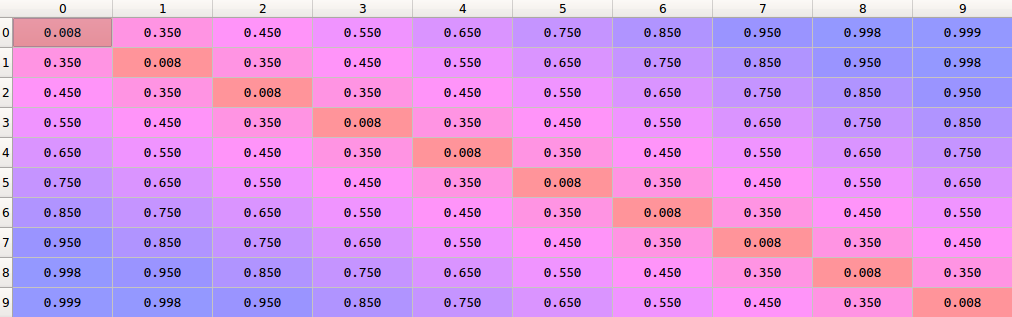
\includegraphics[width=14cm]{../plots/path_means3.png}
  \caption{Adversarial network 2 - initial mean edge weights}
  \label{}
  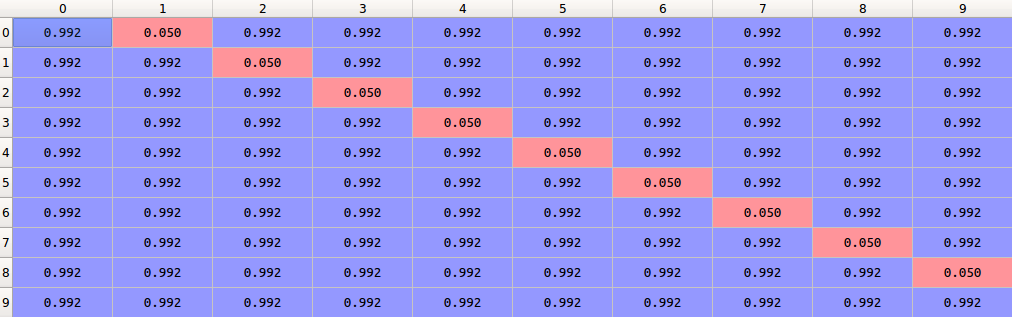
\includegraphics[width=14cm]{../plots/path_means4.png}
  \caption{Adversarial network 2 - second phase mean edge weights}
  \label{}
\end{subfigure}
\caption{Adversarial network 2 mean path weights at each phases}
\label{fig:ullm-particle}
\end{figure}



\subsubsection{Adversarial network 3 - wavelike changes}

In this final adversarial case the mean edge weights increase and decrease gradually over time. Each mean edge weight is essentially a point on a sine wave but shifted up by 1 so that it is always positive and divided by 2 so that the mean edge values fall between 0 and 1. The mean edge weights shift along the sine wave over time so that they gradually increase and decrease. The edges are positioned on the sine wave relative to each other depenent on how close the vertices are which they connect. For example the edges between vertices 1 and 4 and between vertices 5 and 8 will be at the same position on the sine wave (because their vertices are labelled 3 numbers apart), but they will be far away from the edge which connects vertices 2 and 9.\\

The idea of this adversarial case is that it represents gradual shifts over time. Each cycle of the sine wave could be thought of as day and night periods for example, where the edges represent the cost of a communication path. During the days the costly edges would be those which connect businesses which are active during the day, and at night the costly edges switch to those which connect homes which become busy as people return from work.\\

The following table shows the total cost of each algorithm for each of the networks. It also shows the cost for the first 1,000 iterations, the middle 1,000 (when networks 1 and 2 shift) and the last 1,000 to show how each algorithm performs at the different stages.\\


\begin{tabular}{ |p{4.5cm}||p{2.5cm}|p{2.5cm}|p{2.5cm}|p{2.5cm}|  }
 \hline
 \multicolumn{5}{|c|}{Costs of each algorithm over each adversarial network} \\
 \hline
 Network                    & Optimal Path  & CombUCB1  & FPL-TRiX  & TS??  \\
 \hline
 Adversarial network 1      &               &           &           &       \\
  - total cost              & 3,684         & 6,196     & 7,652     &       \\
  - first 1000 iterations   & 450           & 750       & 662       &       \\
  - middle 1000 iterations  & 367           & 845       & 892       &       \\
  - final 1000 iterations   & 286           & 452       & 773       &       \\
 \hline
 Adversarial network 2      &               &           &           &       \\
  - total cost              & 7,244         & 12,447    & 11,890    &       \\
  - first 1000 iterations   & 999           & 1,803     & 1,321     &       \\
  - middle 1000 iterations  & 723           & 1,087     & 1,142     &       \\
  - final 1000 iterations   & 450           & 457       & 1,079     &       \\
 \hline
 Adversarial network 3      &               &           &           &       \\
  - total cost              & 3,844         & 5,482     & 6,262     &       \\
  - first 1000 iterations   & 503           & 809       & 1,007     &       \\
  - middle 1000 iterations  & 178           & 351       & 296       &       \\
  - final 1000 iterations   & 781           & 964       & 1,245     &       \\
 \hline
\end{tabular}\\

In the first adversarial network FPL-TRiX is quicker to identify the long optimal path at the beginning (similar to the result in the stochastic setting). Both algorithms move towards the optimal path in the second phase, but CombUCB1 explores less in this stage which ultimately leads to it returning a lower total cost.\\

The second adversarial framework tries to exploit the fact that CombUCB1 can be slower than FPL-TRiX to adapt to new paths. Indeed this seems to be the case as it performs worse. The cost at the end is less with CombUCB1 but this is a result of the end period being the state with the optimal path that CombUCB1 has got stuck in. Looking at the 1,000 iterations prior to this then CombUCB1's cost is 1,995 and FPL-TRiX's cost is 1,150. Figure XXX shows the progress of the costs of each algorithm over time. It is clear that CombUCB1 goes through phases of slowly increasing cost for 1,000 iterations and then rapidly increasing cost for 1,000 iterations.\\

\begin{figure}[h!]%                 use [hb] only if necceccary!
  \centering
  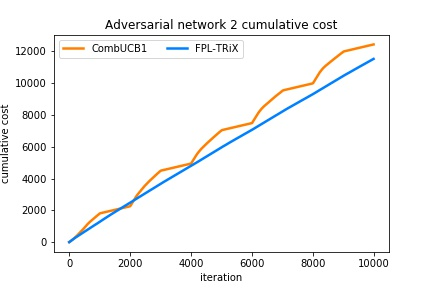
\includegraphics[width=10cm]{../plots/advers_net2_cumul_costs.jpg}
  \caption{Adversarial network 2 - cumulative costs}
  \label{}
\end{figure}

Finally, when the situation is gradually evolving like in the third case, CombUCB1 never becomes too confident on any paths and so it keeps exploring more and performs well again compared to FPL-TRiX.\\


\pagebreak

%----------------------------------------------------------------------------------------
%	PARAMETERS
%----------------------------------------------------------------------------------------

\section{Parameters}

From the analysis so far, some benefits of FPL-TRiX over CombUCB1 are that it can identify optimum paths quicker when the minimum cost path is longer, and that it is less prone to becoming stuck in adversarial situations where the the path distributions change relatively quickly. These advantages rely on the ability to tune the parameters in FPL-TRiX to best suit the situation. In the stochastic setting it is beneficial to adjust the parameters to reduce the amount of exploration the algorithm does. In the adversarial case, however, it should help to keep exploration relatively more active in order to identify when the situation changes and there is a new optimal path. In this section we look at the parameters specifically and understand how changing them affects outcomes.\\

\subsection{Exploration score}

To measure the amount of exploration an algorithm is doing we introduce an "impurity" function. This calculates the proportion of iterations in which each edge is chosen. This value is then multiplied by 1 minus itself (so if the value is p then the calculation is p$\times$(1-p)) and then multiplied by 4 so that the possible values range between 0 and 1. Finally the average of these values is taken over all the edges and multiplied by 1,000 so that the numbers are not tiny.\\

\subsection{Parameters, exploration scores and costs}

To see how the parameters affect exploration and cost let us first observe the performance of FPL-TRiX in the stochastic network. Figure XXX show how the total cost and level of exploration change as the different parameter values change. The main point to note here is that when there is less exploration the algorithm performs better.\\

\begin{figure}[h!]
\centering
\begin{subfigure}{.5\textwidth}
  \centering
  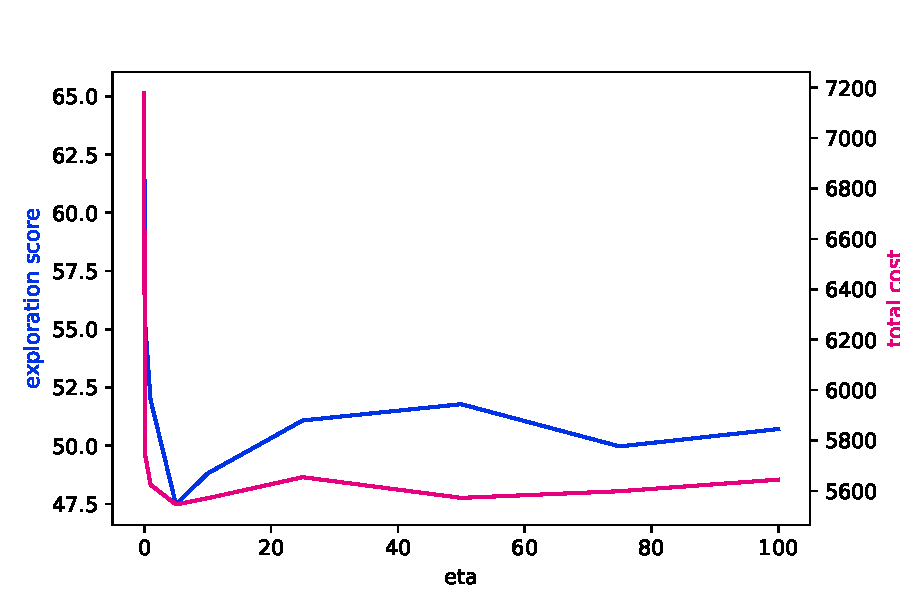
\includegraphics[width=65mm]{../plots/eta_expl_cost.pdf}
\end{subfigure}%
\begin{subfigure}{.5\textwidth}
  \centering
  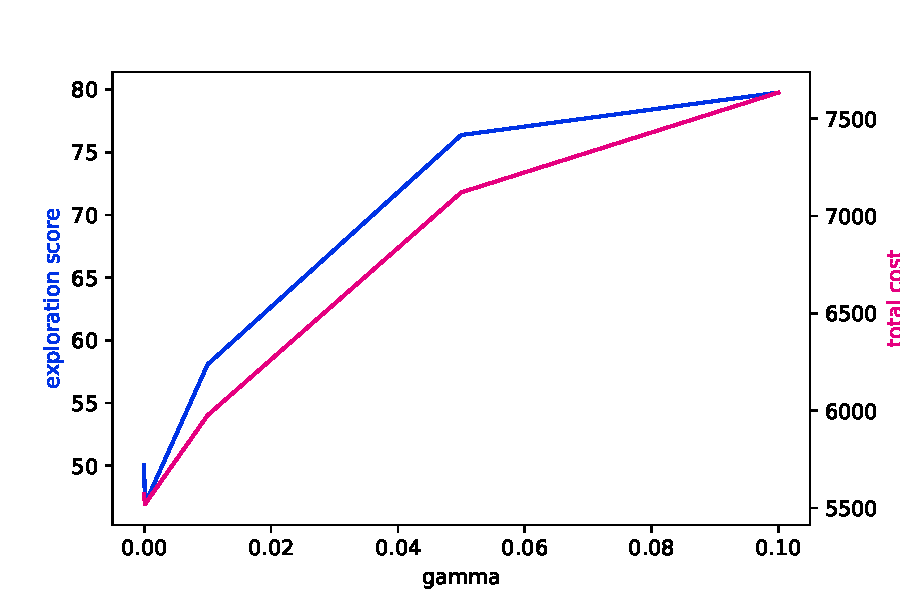
\includegraphics[width=65mm]{../plots/gamma_expl_cost.pdf}
\end{subfigure}
\begin{subfigure}{.5\textwidth}
  \centering
  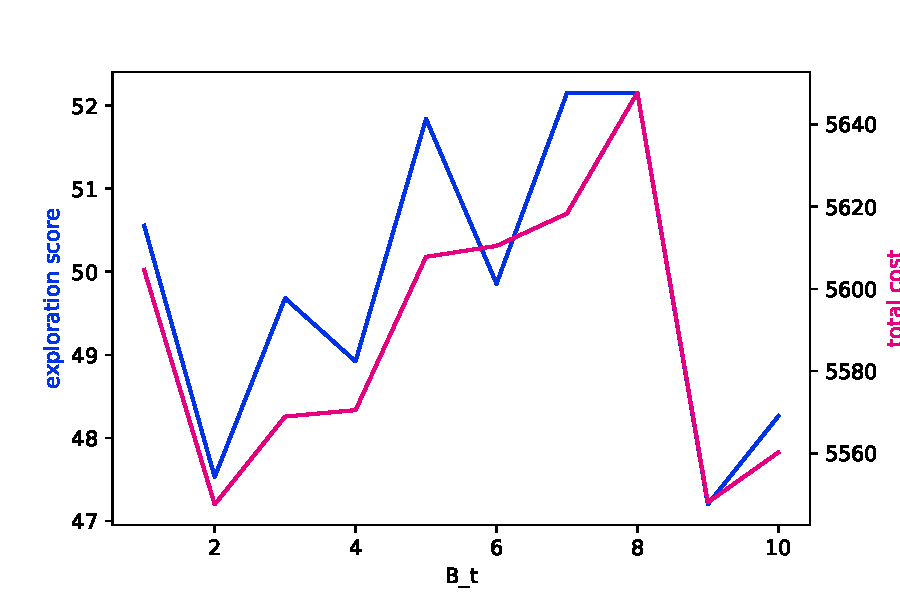
\includegraphics[width=65mm]{../plots/Bt_expl_cost.pdf}
\end{subfigure}
\caption{\textcolor{blue}{Exploration score} and \textcolor{RubineRed}{total cost} for different $\eta$, $\gamma$ and $B_t$}
\label{fig:ullm-particle}
\end{figure}


\subsection{Dynamic $B_t$ parameter}

In Neu 2015 [2] it is proposed that the $B_t$ parameter in FPL-TRiX is non-increasing, but is variable over time. $B_t$ is a control on the amount that the algorithm explores - the higher $B_t$ is the larger the perturbations are able to be and therefore it is more likely for "worse" performing edges to be perturbed to a value where they are chosen in an iteration. Therefore   one idea to improve the performance of FPL-TRiX in adversarial cases is to allow the $B_t$ parameter to adjust to the situation. In particular, if the situation changes then the parameter could be increased to encourage exploration to find a new optimal path, after which the parameter would be decreased again.\\

These parameter adjustments could be carried out with some prior knowledge of the system. For example, for communications networks, this could be at the start and at the end of normal working hours, or at the beginning of seasons or holiday periods. Another way to adjust the parameter could be to allow it to somehow recognise itself when the situation changes. For example if the variance of the reward/cost at each iteration changes.\\

Testing out this idea in the adversarial cases previously discussed, however, bares little fruit. The main reason for this is that $B_t$ makes little to no difference on the outcome of the algorithm. In fact the main effect it has is to increase the variance of the result. This can be observed in figure XXX whereby changing the $B_t$ parameter has a seemingly unpredictable effect on the cost.\\


\subsection{Dynamic $\gamma$ and $\eta$ parameters instead?}

Given that, in practice, the $B_t$ does not have a clearly observable effect on the outcome of FPL-TRiX in an adversarial network, perhaps allowing some of the other parameters to vary could yield better results. Testing the cost at different periods with different $\gamma$ parameters yields the following:\\

\begin{tabular}{ |p{3cm}||p{1.5cm}|p{1.5cm}|p{1.5cm}|p{1.5cm}|p{1.5cm}|  }
 \hline
 \multicolumn{6}{|c|}{Costs at different periods for differnt $\gamma$ parameters}  \\
 \hline
 Cost over  iterations:& 1-1000  & 4000-5000 & 5000-6000 & 9000-10000  & total cost  \\
 \hline
 $\gamma=0.01$        & 694     & 626       & 1,266     & 821         & 8,397       \\
 $\gamma=0.1$         & 725     & 716       & 1,037     & 699         & 7,735       \\
 \hline
\end{tabular}\\

The lower $\gamma$ parameter provides the best results in the early stages but then once the system changes the higher $\gamma$ parameter yields better results. So can changing the $\gamma$ parameter over time reduce the total cost returned? It seems like a parameter of 0.01 performs best at first and then changing to 0.1 is better for the second stage. However, in reality simply changing the parameter in this way does not lead to the best performance here. The behaviour over time of each scenario can be observed in figure XXX.\\

\begin{figure}[h!]
\centering
\begin{subfigure}{1.0\textwidth}
  \centering
  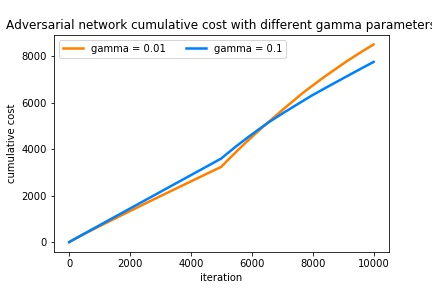
\includegraphics[width=10cm]{../plots/changing_gamma_cumul_cost.jpg}
  \caption{}
  \label{}
\end{subfigure}
\caption{Cumulative cost for different gamma parameters}
\label{fig:ullm-particle}
\end{figure}

The total cost seems to be largely determined by the settings at the initial stages. Although changing the parameter when the adversarial situation changes does appear to be advantageous compared to keeping it at 0.01, it still lags the performance when gamma is set to 0.1 for the entire time. It does, however, suggest that using some sort of changing $\gamma$ parameter could be beneficial in some cases, and indeed in this case the changing parameter model is lowest cost after around 6,000 iterations.

\pagebreak

%----------------------------------------------------------------------------------------
%	THESIS CONTENT - APPENDICES
%----------------------------------------------------------------------------------------

\appendix % Cue to tell LaTeX that the following "chapters" are Appendices

% Include the appendices of the thesis as separate files from the Appendices folder
% Uncomment the lines as you write the Appendices


%\include{Appendices/AppendixB}
%\include{Appendices/AppendixC}

%----------------------------------------------------------------------------------------
%	BIBLIOGRAPHY
%----------------------------------------------------------------------------------------




\end{document}